% ============================================================
% Projective Dynamic Logo (PDL)
% Global Mapping of Structures, Results, and Open Problems
% Version 17 — C. Laubscher
% ============================================================
\documentclass[11pt,a4paper]{article}

% ---- Encoding and fonts ----
% Compiler avec pdflatex (UTF-8 natif via inputenc) ou XeLaTeX
\usepackage[utf8]{inputenc}
\usepackage[T1]{fontenc}
\usepackage{lmodern}

% ---- Page layout ----
\usepackage[margin=2.5cm]{geometry}

% ---- Mathematics ----
\usepackage{amsmath,amssymb,amsthm}

% ---- Tables and lists ----
\usepackage{booktabs}
\usepackage{longtable}
\usepackage{array}
\usepackage{ragged2e}
\usepackage{enumitem}
\newcolumntype{L}[1]{>{\RaggedRight\arraybackslash}p{#1}}

% ---- Graphics ----
\usepackage{graphicx}
\usepackage{float}
\usepackage{tikz}
\usetikzlibrary{positioning,backgrounds,arrows.meta,fit}
\pgfdeclarelayer{background}
\pgfsetlayers{background,main}

% ---- Captions and colours ----
\usepackage[font=small,labelfont=bf]{caption}
\captionsetup[table]{labelsep=quad}
\usepackage{xcolor}
\definecolor{proofblue}{RGB}{0,70,140}
\definecolor{conjecturegreen}{RGB}{0,120,60}
\definecolor{hypothesisorange}{RGB}{200,90,0}
\definecolor{openproblemred}{RGB}{170,0,0}

% ---- Hyperlinks ----
\usepackage{hyperref}
\usepackage{doi}
\usepackage{url}
\hypersetup{
colorlinks=true,
linkcolor=proofblue,
citecolor=proofblue,
urlcolor=proofblue}

% ---- Bibliography ----
\usepackage[numbers,sort&compress]{natbib}

% ---- Theorem environments ----
\theoremstyle{plain}
\newtheorem{theorem}{Theorem}[section]
\newtheorem{proposition}[theorem]{Proposition}
\newtheorem{corollary}[theorem]{Corollary}
\newtheorem{lemma}[theorem]{Lemma}
\theoremstyle{definition}
\newtheorem{definition}[theorem]{Definition}
\newtheorem{axiom}[theorem]{Axiom}
\theoremstyle{remark}
\newtheorem{remark}[theorem]{Remark}
\newtheorem{conjecture}[theorem]{Conjecture}
\newtheorem{openproblem}[theorem]{Open Problem}
\newtheorem{hypothesis}[theorem]{Hypothesis}

% ---- Custom macros ----
\newcommand{\PDL}{\textnormal{PDL}}
\newcommand{\Kfour}{K_4}
\newcommand{\quintuplet}{(24,\,28,\,930,\,10087,\,11017)}
\newcommand{\Geff}{G_{\mathrm{eff}}}
\newcommand{\GPDL}{G_{\mathrm{PDL}}}
\newcommand{\epsG}{\varepsilon_G}
\newcommand{\rval}{r_{\mathrm{val}}}
\newcommand{\Rsurf}{R_{\mathrm{surf}}}
\newcommand{\Rtot}{R_{\mathrm{tot}}}
\newcommand{\sigmaN}{\sigma(N)}
\newcommand{\mustar}{\mu^*}
\newcommand{\SBH}{S_{\mathrm{BH}}}
\newcommand{\Meff}{M_{\mathrm{eff}}}
\newcommand{\MPl}{M_{\mathrm{Pl}}}
\newcommand{\Tpp}{T_{pp}}
\newcommand{\Zsat}{Z_{\mathrm{sat}}}
\newcommand{\Nmin}{N_{\min}}
\newcommand{\epsGeomB}{\varepsilon_G^B}

% ---- List style ----
\setlist[itemize,1]{label=\textendash}
\setlist[itemize,2]{label=\textbullet}

% ============================================================
\title{Projective Dynamic Logo (PDL)\\[4pt]
\large Global Mapping of Structures, Results, and Open Problems\\[2pt]
\normalsize Version 17 --- A Guide for Continuation of the Programme}
\author{C\'edric Laubscher\\[4pt]
\small Independent researcher\\
\small \href{https://cedriclaubscher.ch}{cedriclaubscher.ch}
$\;\cdot\;$
\small \href{https://zenodo.org/communities/pdl-framework/}{zenodo.org/communities/pdl-framework}}
\date{\today}

\begin{document}

\maketitle
\setcounter{tocdepth}{2}

% ============================================================
\begin{abstract}
This document provides a systematic and self-contained guide to the Projective Dynamic Logo (PDL) programme, intended for a scientific colleague who wishes to understand, verify, or continue the research.
PDL is a foundational physics programme that derives fundamental physical constants and dynamical laws from four axioms on finite signed graphs, without presupposing spacetime, particles, or fields.
The minimal admissible closure under the axioms is the complete signed graph $\Kfour$ on four vertices and six edges, identified with the electron prototype.
The proton is characterised by a unique integer quintuplet $\quintuplet$, from which all results flow.

The current corpus (D01--D45, plus auxiliary documents) has reached the following state:
\begin{itemize}
\item Three critical Gates have been resolved: the axiomatic derivation of the amplitude $155/11017$ (Gate~1, D29), the structural proof that the QCD correction coefficient equals~2 (Gate~2, D30), and the theorem $\Geff(N)=\sigmaN\cdot\GPDL$ (Gate~3, D31/D36).
\item Four fundamental dynamical equations have been derived from the $(A)\wedge(B)$ coupling criterion: the Schr\"odinger equation (D32), the Dirac equation (D33), Born's rule via Gleason uniqueness (D34), and the Einstein coupling equation (D35).
\item Newton's gravitational constant $G$ is now a theorem, modulo a single irreducible external parameter ($\Delta m_{\mathrm{iso}} = m_d - m_u$).
\item The Hubble tension is resolved at $0.006\%$ with zero free parameters (D35/D27).
\item Black hole thermodynamics has been derived from PDL axioms: the area law $S \propto \Rsurf$ is an unconditional theorem (D37), and the Bekenstein--Hawking formula $\SBH/k_B = 4\pi(\Meff/\MPl)^2$ follows algebraically from Gate~3 (D38).
\item Open Problem~OP1 has been fully resolved by D42: the Indifference Lemma~H3 is now an unconditional theorem of axioms~C1--C4. As a corollary, $\kappa = 310\varphi/11017 \in \mathbb{Q}(\sqrt{5})$ is promoted to an unconditional theorem of C1--C4, and the entire derivation chain from axioms to the Bekenstein--Hawking entropy is fully axiomatic with no residual free parameter.
\item D40 derives the complete architecture of nuclear stability from the proton and neutron quintuplets alone: $\Nmin(Z) = Z$ for $Z \leq 20$ as an exact theorem, the conflict saturation $C(Z>20) = 190\,\Tpp$ exactly, and the valley of stability reproduced at $100\%$ accuracy for all $Z=1$ to $82$.
\item D41 confronts the PDL framework with the experimental results of Ha et al.\ (\textit{Nature Communications} 16, 10631, 2025), confirming the structural identity $T \approx (\Delta n+1)^2 = 25$ across three independent observables, with the wave-function component ratio agreeing at the $2\%$ level.
\item D43 establishes the computational infrastructure of the programme and proves the geometric leakage parameter $\varepsilon_{\mathrm{geom}}(p) = 329/10087$ as an unconditional theorem (OP-A resolved).
\item D44 derives the hierarchical filter factor $k = 0.921716$ from C1--C4 as an unconditional theorem (OP-B resolved). The complete causal chain C1--C4 $\to$ $K_4$ $\to$ quintuplet $\to$ $\varepsilon_{\mathrm{geom}}$ $\to$ $\varepsilon_G = \varepsilon_{\mathrm{geom}} \times k^{18}$ $\to$ $G$ is now fully closed with no remaining open problem and no free parameter beyond $\Delta m_{\mathrm{iso}}$.
\item D45 derives the first falsifiable astrophysical confrontation: the primordial black hole survival threshold is shifted upward by $+11.89\%$ relative to the standard GR value, giving $M^*_{\mathrm{PDL}} = \sigma(40)^{-2/3}\,M^*_{\mathrm{GR}} \approx 5.706 \times 10^{14}$\,g, testable with existing Fermi-LAT data via \textsc{BlackHawk} and \textsc{Isatis}.
\end{itemize}
There is no longer any foundational open problem at the axiomatic level. The remaining open problems (OP2--OP17) concern higher-level derivations, extensions, and experimental confrontations.
\end{abstract}

\tableofcontents

% ============================================================
\section{Purpose and Scope}
\label{sec:purpose}

\subsection{Aim of this document}
\label{subsec:aim}
This mapping document pursues four objectives. First, it provides a complete and current inventory of the PDL corpus (D01--D45, plus auxiliary documents), with concise descriptions of each document's role and main result. Second, it makes explicit the logical dependency structure of the programme: which results follow from which, what has been proved, and what remains conjectural or open. Third, it classifies all results according to a rigorous epistemic taxonomy, distinguishing proved theorems, conditional theorems whose hypotheses are explicitly named, structurally motivated conjectures, and open problems. Fourth, it identifies the most productive entry points and continuation paths for a colleague wishing to extend the programme. This document is not a replacement for the primary technical documents; it is a navigational and epistemic guide that complements them.

\subsection{What makes this version different from v16}
\label{subsec:diffv16}
Version~16 of the mapping document covered the corpus up to D43 and established the computational infrastructure of the programme via 50-decimal-precision Python/SymPy verification. The present version~v17 incorporates two additional documents (D44 and D45) and marks the closure of the causal chain.

\begin{itemize}
\item D44 resolves OP-B: the hierarchical filter factor $k = 0.921716$ is derived from axioms C1--C4 as an unconditional theorem, via the trace structure of $K_4$ and the $S_4$-equivariance constraints of D42. As a corollary, OP8 (the 17~ppm residual of D28) is simultaneously resolved: the residual reflects the precision of the CODATA measurement of $G$, not a structural gap. The complete causal chain C1--C4 $\to$ $K_4$ $\to$ quintuplet $\to$ $\varepsilon_{\mathrm{geom}}$ $\to$ $\varepsilon_G = \varepsilon_{\mathrm{geom}} \times k^{18}$ $\to$ $G$ is now closed with no remaining open problem.
\item D45 formulates the first falsifiable confrontation of the PDL framework with astrophysical data. The prediction $M^*_{\mathrm{PDL}} = \sigma(40)^{-2/3}\,M^*_{\mathrm{GR}} \approx 5.706 \times 10^{14}$\,g is an unconditional corollary of the density-dependent gravitational coupling, and implies a non-zero Hawking radiation excess at $E_{\mathrm{peak}} \approx 90$--$104$\,MeV in the isotropic gamma-ray background. The document identifies the precise test using \textsc{BlackHawk} and \textsc{Isatis} together with Fermi-LAT data.
\end{itemize}

The reader familiar with v16 should note the following epistemic changes: OP-B and OP8 are now resolved (moved to the resolved list); the ``Recommended next documents'' section has been updated to reflect the new frontier; the Falsifiable Predictions table gains entry P5-bis (spectral cutoff position) and the Corpus Inventory gains two rows. The dependency map gains a D45 node connected from BH entropy (D38).

\subsection{Epistemic conventions}
\label{subsec:conventions}
Throughout this document, the following colour-coded epistemic labels are used in tables and text:
\begin{description}[leftmargin=2.5cm, style=nextline]
\item[\textcolor{proofblue}{Theorem}] A result established by a complete proof from the PDL axioms C1--C4 and previously proved theorems, with no free parameters and no unproved auxiliary hypotheses.
\item[\textcolor{proofblue}{Theorem (H$x$)}] A result proved under one or more explicitly named hypotheses H1, H2, H3\ldots; the proof itself is complete conditional on those hypotheses.
\item[\textcolor{conjecturegreen}{Conjecture}] A structurally motivated claim supported by numerical evidence, qualitative arguments, or partial proofs, but not yet established rigorously.
\item[\textcolor{hypothesisorange}{Named Hypothesis}] An auxiliary assumption that is explicitly labelled and isolated, so that results depending on it are clearly traceable.
\item[\textcolor{openproblemred}{Open Problem}] A well-posed question whose resolution would advance the programme significantly.
\end{description}

% ============================================================
\section{Document Corpus}
\label{sec:corpus}

\subsection{Complete document table}
\label{subsec:doctable}
Table~\ref{tab:documents} lists the complete PDL corpus in Zenodo canonical order.

\begin{longtable}{L{1.3cm}L{3.8cm}L{8.0cm}}
\caption{PDL corpus in Zenodo canonical order. \emph{Main result} denotes the single most consequential contribution of each document to the programme chain.}
\label{tab:documents}\\
\toprule
\textbf{Label} & \textbf{Title (abbreviated)} & \textbf{Main result / role}\\
\midrule
\endfirsthead
\toprule
\textbf{Label} & \textbf{Title (abbreviated)} & \textbf{Main result / role}\\
\midrule
\endhead
\bottomrule
\endfoot
D01 & The Emergence of Physical Reality within the PDL Framework~\cite{D01} & Founding article: four relational axioms, structure, proton architecture, first treatment of $\alpha$, $\mu$, $G$, and cosmology.\\[0.3em]
D02 & Introduction to the PDL~\cite{D02} & High-level conceptual overview; standard first reading for new collaborators.\\[0.3em]
D01F & L'\'emergence de la r\'ealit\'e physique (LDP FR)~\cite{D01F} & French translation of D01.\\[0.3em]
D03 & The Emergence of Physical Reality (IMRaD format)~\cite{D03} & Journal-formatted version of D01.\\[0.3em]
D04 & A Modal Dialogue between PDL and the Theory of Objectivity~\cite{D04} & Comparative study of PDL and TO; ontological commitments of PDL.\\[0.3em]
D05 & A Minimal Relational Sketch for the Golden Ratio in PDL~\cite{D05} & Self-similar core--surface partition; golden ratio and active surface $(\sigma,3)$.\\[0.3em]
D06 & Hierarchical Filtering of Coherence Leakage and the Exponent~18~\cite{D06} & First formulation of the 18-filter leakage hierarchy.\\[0.3em]
D07 & Gleason-Type Uniqueness of Born's Rule for Spin-$\tfrac{1}{2}$~\cite{D07} & Early sketch of the Gleason approach; superseded by D34 at Level~1.\\[0.3em]
D08 & Logical Leakage as Self-Maintained Probability: Topological Reformulation~\cite{D08} & Coexistence topology; coherence-cost pseudo-metric; leakage as probability.\\[0.3em]
D09 & PDL as a Foundational Research Programme~\cite{D09} & Programme position paper; first systematic open-problem list.\\[0.3em]
D10 & From Discrete Coherence Flux to Effective Fields~\cite{D10} & Gauss- and Faraday-like relations from coherence fluxes; path towards Schr\"odinger.\\[0.3em]
D10a & Proper Time as Coherence-Cycle Counting~\cite{D10a} & Proper time as a count of coherence cycles; emergent Minkowski structure.\\[0.3em]
D11 & Towards an Einstein--Dirac Unification from PDL~\cite{D11} & Preliminary sketch coupling Dirac spinors to the emergent coherence-cost metric.\\[0.3em]
D12 & A Structural Derivation of the Fine-Structure Constant from PDL~\cite{D12} & Closed-form expression for $\alpha$ from $(930, \sigma, \varphi)$; accuracy $\mathcal{O}(10^{-4})$.\\[0.3em]
D13 & Compatibility of the Schr\"odinger Framework with PDL~\cite{D13} & Benchmark: PDL-derived $\alpha$ and $\mu$ in hydrogenic Schr\"odinger; spectral concordance.\\[0.3em]
D14 & Born's Rule and the Golden-Ratio Active Surface in PDL~\cite{D14} & Relational derivation of Born's rule for spin-$\tfrac{1}{2}$; role of $\varphi$ in $\sigma$.\\[0.3em]
D15 & Towards a Schr\"odinger-Type Dynamics from PDL: A Relational Sketch~\cite{D15} & Early sketch of Schr\"odinger emergence; superseded by D32.\\[0.3em]
D16 & Combinatorial Selection of the Proton Architecture: Uniqueness Conjecture~\cite{D16} & Optimisation functional for the quintuplet; local uniqueness conjecture.\\[0.3em]
D16a & Minimal Stationary Closures in PDL: Necessity of the $(4,6)$ Block~\cite{D16a} & \textcolor{proofblue}{Theorem}: no admissible closure exists on $|V|<3$; $K_4$ is first admissible.\\[0.3em]
D16b & Combinatorial Selection and Local Uniqueness of the Proton Architecture~\cite{D16b} & Refined combinatorial treatment; local uniqueness conjecture for $\quintuplet$.\\[0.3em]
D17 & Coherence Leakage, Hierarchical Filtering, and the Exponent~18~\cite{D17} & Organisation of the 18 filters into three blocks; effective coupling ansatz $\varepsilon^{18}$.\\[0.3em]
D18 & Discrete Cavity Modes and Logical Density of States~\cite{D18} & PDL cavity modes; $2n^2$ density-of-states in three dimensions.\\[0.3em]
D19 & Existence as Pulsating Closure: An Ontological Meditation~\cite{D19} & Philosophical analysis of PDL boundaries, leakage, and transcendence.\\[0.3em]
D20F & Qui que nous puissions \^etre (FR)~\cite{D20F} & French philosophical synthesis; companion to D20.\\[0.3em]
D20 & Whoever We May Be: A Philosophical Synthesis of PDL~\cite{D20} & Ontological and existential synthesis; accessible entry point for non-specialists.\\[0.3em]
D21 & Universal Coherence Leakage: A Structural Bridge between $G$ and $V_3$~\cite{D21} & \textcolor{proofblue}{Primary result}: $R_{\mathrm{tot}}/R_{\mathrm{surf}} = 2\nu^2/(2\nu^2-1)$; $G \approx 6.67448\times 10^{-11}$ m$^3$kg$^{-1}$s$^{-2}$ (27~ppm vs.\ CODATA~2022).\\[0.3em]
DN & \emph{Whatever We May Be}: The PDL popular book~\cite{DN} & Popular science monograph; non-technical introduction to PDL.\\[0.3em]
D22 & Nuclear Stability and the Periodic Table as Combinatorial Closure Hierarchies~\cite{D22} & Neutron quintuplet $(24,28,1032,9960,10992)$; $N_{\mathrm{crit,max}}=126.1$; $Z_{\mathrm{sat}}=20$.\\[0.3em]
DM & PDL Global Mapping v17~\cite{DMapv10} & Navigation document for the complete corpus D01--D45; the present document.\\[0.3em]
D23 & Topological Origin of the Exponent~18, $S^2$, and the Periodic Table~\cite{D23} & \textcolor{proofblue}{Theorem}: $18=6+5+4+3$ is topologically necessary via $S^2$; common ancestor of exponent~18 and the periodic table.\\[0.3em]
D24 & Closure-Density Dependence of $\kappa$ and the Hubble Tension~\cite{D24} & Introduction of $\sigma(N)=1-(1-\kappa)^N$; structural origin of $H_0$ discrepancy.\\[0.3em]
D25 & A Parameter-Free Structural Bridge between $\alpha$ and $G$~\cite{D25} & \textcolor{proofblue}{Primary result}: full bridge formula; $G$ at 27~ppm; $\kappa\approx 0.0075194$.\\[0.3em]
D26 & Cosmological Resolution via PDL: $G$ as Topology-Dependent~\cite{D26} & $G$ as topology-dependent parameter; Hubble tension as scale-transition signature.\\[0.3em]
D27 & Structural Derivation of $N_{\mathrm{CMB}}$ from the PDL Neutron Architecture~\cite{D27} & $N_{\mathrm{CMB}}=40$ from $n_6$; $n_{-}$; $H_{0,\mathrm{CMB}}=67.26$ km\,s$^{-1}$\,Mpc$^{-1}$; $0.27\sigma$ Planck.\\[0.3em]
D28 & The PDL--QCD Boundary: Mass Ratio, Correction, and the $\epsGeomB$ Conjecture~\cite{D28} & $\mu = \frac{155}{11017}(1-2\kappa^2)\frac{m_{\mathrm{iso}}}{m_p}$; $\epsGeomB$ conjecture formulated.\\[0.3em]
D29 & Axiomatic Derivation of $155/11017$: Gate~1 Resolved~\cite{D29} & \textcolor{proofblue}{Theorem}: $155/11017$ proved from C1--C4 via AB; $768/768$ exhaustive verification.\\[0.3em]
D30 & QCD Correction Coefficient $a=2$: Gate~2 Resolved~\cite{D30} & \textcolor{proofblue}{Theorem}: $a=2$ structurally forced; $m_{\mathrm{iso}}=m_d-m_u$ is the unique irreducible external parameter.\\[0.3em]
D31 & Proof of $\Geff(N)=\sigmaN\cdot\GPDL$: Gate~3 (preliminary)~\cite{D31} & First proof of Gate~3 under linear bridge inversion hypothesis; superseded in rigour by D36.\\[0.3em]
D32 & Schr\"odinger Dynamics from the AB Coupling Criterion~\cite{D32} & \textcolor{proofblue}{Theorem}: Schr\"odinger equation derived; $b=-i\hbar/(2m_e)$; $\partial_x^2$ forced by AB.\\[0.3em]
D33 & Dirac Equation from the $\mathrm{SL}(2,\mathbb{C})$ Pulsation of $K_4$~\cite{D33} & \textcolor{proofblue}{Theorem}: $T=-i\sigma_2$ unique among 8 candidates; $T^2=-I_2$; Clifford algebra; NR limit = D32 exactly.\\[0.3em]
D34 & Born Rule from AB-Admissible Amplitudes~\cite{D34} & \textcolor{proofblue}{Theorem} Level~1: five Gleason axioms verified; Born rule unique from Gleason uniqueness.\\[0.3em]
D35 & Quantitative Einstein Equation from $\sigmaN$~\cite{D35} & \textcolor{proofblue}{Theorem (H1)}: $G_{\mathrm{eff}}(N)=G_{\mathrm{Newton}}$; Hubble ratio at $0.006\%$; synthesis document.\\[0.3em]
D36 & Proof of $\Geff(N)=\sigmaN\cdot\GPDL$ from the Trace Structure of $K_4$~\cite{D36} & \textcolor{proofblue}{Theorem (H1)}: $\sigma_0=0$ exact from AB; $\mathrm{Tr}(A)=0$ proved; hypothesis reduced to H1 alone; Gate~3 strengthened.\\[0.4em]
D37 & Surface Locality of Relational Entropy and the PDL Area Law~\cite{D37} & \textcolor{proofblue}{Theorem BH-1}: entropy of a PDL closure is entirely carried by $\Rsurf$; area law $S\propto\Rsurf$ unconditional.\\[0.3em]
D38 & Bekenstein--Hawking Entropy from the PDL Effective Gravitational Coupling~\cite{D38} & \textcolor{proofblue}{Theorem BH-2} (under H1): $\SBH/k_B=4\pi(\Meff/\MPl)^2$; verified to $10^{-15}$; three falsifiable PBH predictions.\\[0.3em]
D39 & Derivation of $\kappa$ from the PDL Axioms: the Indifference Lemma~\cite{D39} & \textcolor{proofblue}{Theorem (H3)}: $\kappa=3/\sigma$ under H3; partial resolution of OP1; D36~$\Rightarrow$~H3 is the unique residual.\\[0.4em]
D40 & Nuclear Stability and the Periodic Table from PDL Combinatorial Axioms~\cite{D40} & \textcolor{proofblue}{Theorems}: $N_{\min}(Z\leq20)=Z$ exact; $C(Z>20)=190\,\Tpp$ exact; valley of stability at $100\%$ for $Z=1$--82; eight assembly rules; connection identified between OP14 (sub-shell filling rates) and OP12 (BH coefficient $\tfrac{1}{4}$).\\[0.4em]
D41 & Structural Closure Multiplicity and the Isospin-Symmetric Island of Inversion~\cite{D41} & First PDL confrontation with nuclear spectroscopy data (Ha et al.~2025). Three independent observables consistent with $T=({\Delta n}+1)^2=25$: $\mathrm{BE2}$ ratio ($22\%$); $N_{\mathrm{comp}}(^{86}\mathrm{Mo})/N_{\mathrm{comp}}(^{84}\mathrm{Mo})=1.962$ vs.\ PDL $2.000$ ($2\%$); $\Delta S_{WF}$ ($25\%$). Closure multiplicity conjecture $H_B$ introduced. Two falsifiable predictions for $^{88}$Ru/$^{90}$Ru and $^{92}$Pd/$^{94}$Pd. ZBM3--PDL correspondence conjectured.\\[0.4em]
D42 & Derivation of H3 from Axioms C1--C4: The Equiparticipation Lemma~\cite{D42} & \textcolor{proofblue}{Theorem}: H3 (Indifference Lemma) derived from C1--C4 without additional input, via three lemmas: D42-L1 (Equiparticipation; C4-optimal $\Rightarrow$ uniform participation $n-2$ per edge, exhaustively verified for $n=4$--7), D42-L2 (cross-triangle blindness, from D39), D42-L3 ($S_4$-equivariance of cross-edge coherence, $24{,}576$ cases, zero violations). Corollary: $\kappa=310\varphi/11017\in\mathbb{Q}(\sqrt{5})$ is an unconditional theorem of C1--C4. OP1 fully resolved.\\[0.4em]
D43 & Numerical Verification of the PDL Causal Chain: 18-Filter Architecture and Colab Infrastructure~\cite{D43} & First systematic numerical verification of the PDL chain at 50-decimal precision (Python/SymPy). Organises the 18 filters into four functional groups (Group~0: axioms; Group~I: constants; Group~II: dynamics; Group~III: thermodynamics). Proves $\varepsilon_{\mathrm{geom}}(p) = 329/10087$ and $\varepsilon_{\mathrm{geom}}(n) = 468/9960$ as unconditional theorems (OP-A resolved). Provides reusable Colab code for all core PDL quantities.\\[0.4em]
D44 & Closure of OP-B: Derivation of the Hierarchical Filter Factor $k$ from the PDL Axioms~\cite{D44} & \textcolor{proofblue}{Theorem}: $k = 0.921716$ derived from C1--C4 via the trace structure of $K_4$ and $S_4$-equivariance constraints of D42 (unconditional). Corollary: OP8 resolved --- the 17~ppm residual of D28 reflects CODATA precision on $G$, not a structural gap. The complete causal chain C1--C4 $\to$ $K_4$ $\to$ quintuplet $\to$ $\varepsilon_{\mathrm{geom}}$ $\to$ $\varepsilon_G = \varepsilon_{\mathrm{geom}} \times k^{18}$ $\to$ $G$ is fully closed. OP-B resolved.\\[0.4em]
D45 & Primordial Black Hole Evaporation Threshold from PDL: A Falsifiable Prediction for Fermi-LAT~\cite{D45} & First falsifiable astrophysical confrontation. $M^*_{\mathrm{PDL}} = \sigma(40)^{-2/3} M^*_{\mathrm{GR}} \approx 5.706 \times 10^{14}$\,g ($+11.89\%$), unconditional corollary of D38 and D42. Excess Hawking flux at $E_{\mathrm{peak}} \approx 90$--$104$\,MeV in the IGRB. Test protocol identified: \textsc{BlackHawk} + \textsc{Isatis} + Fermi-LAT IGRB data (Ackermann et al.\ 2015). AGN $S/E$ redshift trend (DESI/Euclid) as complementary observable.\\[0.4em]
\end{longtable}

\subsection{Reading guide for a new collaborator}
\label{subsec:readingguide}
The following reading pathways are recommended depending on one's entry point.

\begin{itemize}
\item \textbf{Understanding the foundations.} Start with D02 (conceptual overview), then D16a (proof that $K_4$ is the unique minimal closure), then D01 (full axiomatic development). For the proton architecture, read D16 and D16b for the combinatorial selection arguments.
\item \textbf{Understanding the constants.} Read D12 for $\alpha$, then D21 and D25 for the $\alpha$--$G$ bridge. Read D23 for the topological proof that the exponent~18 is necessary. Then read D29 and D30 for the Gate~1 and Gate~2 proofs. Read D36 for the final Gate~3 proof, and D39/D42 for the full resolution of OP1.
\item \textbf{Understanding the dynamics.} Read D32 (Schr\"odinger), D33 (Dirac), D34 (Born), D35 (Einstein) in order.
\item \textbf{Understanding the cosmology.} Read D24, D27, and D35.
\item \textbf{Understanding black hole thermodynamics.} Read D37 (area law), then D38 (Bekenstein--Hawking and PBH predictions), then D45 (falsifiable confrontation with Fermi-LAT).
\item \textbf{Understanding nuclear stability and the periodic table.} Read D22, D23, D40, and D41.
\item \textbf{The closure of the foundational programme.} Read D39 first for context, then D42 for the full proof of H3. After D42, all results previously conditional on H3 are unconditional theorems. Then read D43 (geometric leakage, OP-A) and D44 (filter factor $k$, OP-B) for the complete causal chain to $G$.
\item \textbf{Numerical verification and the computational infrastructure.} Read D43. It provides self-contained Colab code for every major result and defines the verification protocol for future documents.
\item \textbf{Continuing the programme.} Read Section~\ref{sec:openproblems} for the complete prioritised list of open problems, and Section~\ref{sec:dependency} for the critical-path dependency map.
\end{itemize}

% ============================================================
\section{Axiomatic Foundations}
\label{sec:axioms}

\subsection{The four relational axioms C1--C4}
\label{subsec:axioms}
A logical configuration in PDL is a finite signed graph $G=(V,E,s)$, where $V$ is a finite set of vertices (informational entities), $E$ is a set of undirected edges (binary relations), and $s\colon E\to\{1,-1\}$ assigns a sign (agreement or disagreement) to each relation~\cite{D01,D02}. Four relational axioms are imposed.

\begin{axiom}[C1 --- Minimal binary pulsation]
Existence is instantiated as a repeatable, non-trivial alternation between two discrete states, independent of any pre-existing temporal metric. Formally, the discrete dynamical system defined on the space of sign configurations must admit at least one logical $2$-cycle: a configuration that returns to itself after exactly two update steps and is not a fixed point.
\end{axiom}

\begin{axiom}[C2 --- Triangular coherence]
Closed triples of edges (triangles) constitute the elementary coherence motifs. Each triangle contributes to a stability functional according to the product of its three edge signs: a triangle is \emph{coherent} if the product equals $+1$ (balanced) and \emph{violated} if the product equals $-1$ (frustrated).
\end{axiom}

\begin{axiom}[C3 --- Minimal completeness]
The configuration must be self-sufficient: it admits no non-trivial decomposition into independent sub-configurations that satisfy C1 and C2 separately. Formally, the underlying graph must be connected and its coherence structure non-reducible.
\end{axiom}

\begin{axiom}[C4 --- Logical optimisation]
Among all configurations satisfying C1--C3, those that are physically instantiated are those that minimise the coherence cost (fraction of violated triangles) for a given number of vertices and edges.
\end{axiom}

\subsection{The minimal admissible closure \texorpdfstring{$K_4$}{K4}}
\label{subsec:K4}
\begin{theorem}[\cite{D16a}]
\label{thm:K4}
No finite signed graph on $|V|<3$ vertices satisfies all four axioms C1--C4 simultaneously. The complete signed graph on $|V|=4$ vertices and $|E|=6$ edges, denoted $\Kfour$, is the first admissible elementary stationary closure. It is minimal (no proper sub-closure satisfies C1--C4) and quasi-unique (the sign pattern is unique up to the global symmetry group $S_4$).
\end{theorem}

The dynamical interpretation is as follows: $\Kfour$ undergoes a logical $2$-cycle in which edge signs are updated according to a coherence-minimisation rule. This cycle is identified with the Compton oscillation of the electron at rest, and the coherence cost per cycle is identified with $\hbar\omega_C$, making $\hbar$ the minimal quantum of action~\cite{D01,D02}. The dimensionality $n=3$ of physical space is structurally selected: the condition $E_{\mathrm{shell}}\sim S_{\mathrm{shell}}^n$ holds if and only if $n\in\{1,3\}$~\cite{D23}.

\subsection{Three spatial dimensions from \texorpdfstring{$S^2\cong S^2$}{S² ≅ S²}}
\label{subsec:topology}
\begin{theorem}[\cite{D23}]
\label{thm:exponent18}
$K_4$, equipped with its four triangular faces, is homeomorphic to $S^2\subset\mathbb{R}^3$. The homology $H_2(S^2)\cong\mathbb{Z}\oplus\mathbb{Z}$ imposes a rank deficit of exactly one at each hierarchical transition of the PDL chain complex, yielding the unique decomposition $18=6+5+4+3$. The exponent~18 in $\varepsilon^{18}$ is therefore a topological necessity, not a free counting choice. The kernel of the proton-to-nuclear transition map is $d_1=\varepsilon_p/930$ over $\mathbb{Q}(\sqrt{5})$, meaning that the proton valence content $p=930$ does not propagate to the nuclear level. The common topological ancestor of this exponent and the maximum electron count $2\times 6\times 1=18$ per period of the periodic table is the two-sphere $S^2$.
\end{theorem}

% ============================================================
\section{The Proton Architecture}
\label{sec:proton}

\subsection{The integer quintuplet}
\label{subsec:quintuplet}
The proton is the minimal hierarchical composite closure---the smallest structure that can be assembled from $K_4$ blocks and satisfy C1--C4 at a higher level of organisation. It is uniquely characterised by the integer quintuplet $\quintuplet$, where
\begin{itemize}
\item $\nu_u = 24$: the number of coherence cycles in the proton's valence core,
\item $\nu_d = 28$: the number of coherence cycles in the proton's mixed-sign core,
\item $\sigma = 930$: the number of valence coherence relations (active surface $R_{\mathrm{surf}}$),
\item $R_{\mathrm{sea}} = 10087$: the number of sea coherence relations,
\item $R_{\mathrm{tot}} = 11017$: the total number of coherence relations ($R_{\mathrm{surf}}+R_{\mathrm{sea}}$).
\end{itemize}
The active surface is $\sigma=(\varphi,3)$, where $\varphi=\tfrac{1+\sqrt{5}}{2}$ is the golden ratio, arising from the self-similar core--surface partition~\cite{D05,D12}.

\subsection{Combinatorial selection}
\label{subsec:combinatorial}
The quintuplet is selected by a combination of structural constraints arising from C1--C4 and an optimisation functional that minimises leakage while maximising the active-surface fraction. The local uniqueness conjecture---that $\quintuplet$ is the unique admissible tuple in a neighbourhood of the optimum---has been verified computationally and partially proved~\cite{D16,D16b}. A full algebraic proof of global uniqueness remains open.

\begin{conjecture}[\cite{D16b}]
\label{conj:uniqueness}
The proton quintuplet $\quintuplet$ is the unique integer tuple satisfying all structural constraints imposed by C1--C4 and achieving a local minimum of the coherence leakage functional.
\end{conjecture}

% ============================================================
\section{Fundamental Constants}
\label{sec:constants}

\subsection{The fine-structure constant \texorpdfstring{$\alpha$}{alpha}}
\label{subsec:alpha}
\begin{theorem}[\cite{D12,D25}]
\label{thm:alpha}
The fine-structure constant is given by the surface-to-volume coherence ratio $\alpha^{-1}=(\sigma,3)/\varepsilon$, where $(\sigma,3)=310$ and $\varepsilon\approx 0.0497507$ is the electromagnetic valence surplus. This expression is parameter-free and achieves agreement with $\alpha^{-1}\approx 137.035999$ at the level $\mathcal{O}(10^{-4})$.
\end{theorem}

\subsection{The reduced Planck constant \texorpdfstring{$\hbar$}{hbar}}
\label{subsec:hbar}
The reduced Planck constant is identified as the minimal quantum of action associated with one internal coherence cycle of the $K_4$ closure $E=\hbar\omega_C$, where $\omega_C$ is the pulsation frequency of the electron's logical $2$-cycle~\cite{D01,D02}. This identification is a \textcolor{conjecturegreen}{tightly constrained physical conjecture}: the structural form is fixed by the axioms, but the numerical value of $\omega_C$ is externally calibrated.

\subsection{The gravitational constant \texorpdfstring{$G$}{G}}
\label{subsec:G}
The route from the axioms to $G$ is the deepest result of the current programme; it passes through three Gates.

\paragraph{The leakage parameter $\kappa$.} The proton's integer architecture realises a minimal frustration density on the partition $(\sigma, R_{\mathrm{sea}})=(930, 10087)$, characterised by a primary leakage parameter $\kappa$. The $18$-fold hierarchical filtering (Theorem~\ref{thm:exponent18}) yields the dimensionless gravitational coupling $\kappa_G=G\,m_p^2\,c/\hbar\approx\kappa^{18}$. The bridge formula~\cite{D21,V3D21} and its parameter-free refinement~\cite{D25,D25} establish $\kappa\approx 0.0075194$, $G\approx 6.67448\times10^{-11}$ m$^3$\,kg$^{-1}$\,s$^{-2}$ (27~ppm vs.\ CODATA~2022).

\paragraph{The mass-ratio correction.} The proton--electron mass ratio correction is $\mu=\frac{155}{11017}(1-2\kappa^2)\frac{m_{\mathrm{iso}}}{m_p}$, where $m_{\mathrm{iso}}=m_d-m_u$ is the isospin mass splitting~\cite{D28}.

\paragraph{Named hypotheses for Gate~3.}
\begin{hypothesis}[H1 --- Surface-fraction formula]
$\kappa=\sigma/R_{\mathrm{tot}}$, i.e., the cosmological coupling constant equals the surface-to-total coherence ratio of the proton.
\end{hypothesis}
\begin{hypothesis}[H2 --- Bridge linearity]
The relation between $\kappa$ and $G$ is linear $G=\lambda\kappa$, for a structural constant $\lambda$ determined by the quintuplet.
\end{hypothesis}
\begin{hypothesis}[H3 --- Indifference Lemma \textcolor{proofblue}{(now a theorem, D42)}]
The probability measure on the relations of a PDL closure is uniform. Equivalently, in the absence of any external distinction between relations (as imposed by C3 and C4), no relational subset is \emph{a priori} privileged. This is the unique measure compatible with the $S_4$-symmetry of $K_4$ proved in D36, and has been derived from C1--C4 alone in D42.
\end{hypothesis}

Under H3 (now a theorem), H1 follows as a theorem~\cite{D39}: the two-factor decomposition $\kappa=3/\sigma$ holds. H3 has been derived from C1--C4 in D42 via three lemmas D42-L1, D42-L2, D42-L3; it is no longer a named hypothesis but an unconditional theorem of the programme.

\begin{theorem}[Gate~3, \cite{D36}]
\label{thm:Gate3}
Since H3 is now a theorem~\cite{D42}, H1 follows unconditionally~\cite{D39}, and Gate~3 holds without any named hypothesis: $\Geff(N)=\sigmaN\cdot\GPDL$ and $\sigma_0\equiv 0$. The independence of gravitational engagements ($\sigma_0=0$ exactly) follows from the AB coupling criterion without additional hypothesis. The tracelessness $\mathrm{Tr}(A)=0$ of the generator matrix follows from the combinatorial structure of $K_4$ alone.
\end{theorem}

\subsection{The proton--electron mass ratio \texorpdfstring{$\mu$}{mu}}
\label{subsec:mu}
The PDL prediction for the proton--electron mass ratio is $\mu\approx 1836.152\,670$, a parameter-free result consistent with the experimental value $1836.152\,673\,43(11)$ at the level of $1.8\times10^{-9}$~\cite{D28,D29,D30}. This is the programme's primary near-term falsifiable prediction; current precision measurements can test it at $0.001$~ppm.

% ============================================================
\section{The Three Gates: Critical Proofs}
\label{sec:gates}

\subsection{Gate~1: Axiomatic derivation of \texorpdfstring{$155/11017$}{155/11017}}
\label{subsec:gate1}
\begin{theorem}[Gate~1, \cite{D29}]
\label{thm:Gate1}
The amplitude $155/11017$ appearing in the mass-ratio correction formula is derivable from PDL axioms C1--C4 alone, via the AB coupling criterion. Specifically:
\begin{itemize}
\item The stability criterion AB has been verified exhaustively over all $768$ admissible configurations.
\item In every stable case, $P_2/P_1=-1$ exactly.
\item The combinatorial count yields $155/11017$ without any free parameter.
\end{itemize}
\end{theorem}

\subsection{Gate~2: The QCD correction coefficient \texorpdfstring{$a=2$}{a=2}}
\label{subsec:gate2}
\begin{theorem}[Gate~2, \cite{D30}]
\label{thm:Gate2}
The QCD correction coefficient $a=2$ in the mass-ratio formula $\mu=\frac{155}{11017}(1-2\kappa^2)\frac{m_{\mathrm{iso}}}{m_p}$ is structurally forced by axiom~C1 (minimal binary pulsation): the factor~$2$ counts the two distinct pulsation branches of the proton's valence core. Furthermore, $m_{\mathrm{iso}}=m_d-m_u$ is the unique irreducible external parameter at the PDL--QCD interface; it cannot be derived from C1--C4 alone.
\end{theorem}

\subsection{Gate~3: \texorpdfstring{$\Geff(N)=\sigmaN\cdot\GPDL$}{Geff(N)=sigmaN·GPDL}}
\label{subsec:gate3}
Gate~3 was first established in D31 under a linear bridge inversion hypothesis. D36 strengthened this proof by:
\begin{enumerate}
\item Proving that the independence of gravitational engagements ($\sigma_0=0$) follows exactly from AB, without any additional assumption.
\item Proving that $\mathrm{Tr}(A)=0$ from the combinatorial structure of $K_4$ alone.
\item Reducing the remaining hypothesis to H1 only (H2 was absorbed into the proof).
\end{enumerate}
D39 further reduced H1 to H3: given the Indifference Lemma, H1 follows as a theorem. D42 then proved H3 from C1--C4 unconditionally. See Theorem~\ref{thm:Gate3} for the full statement.

% ============================================================
\section{Derived Dynamical Equations}
\label{sec:dynamics}

\subsection{The Schr\"odinger equation (D32)}
\label{subsec:schrodinger}
\begin{theorem}[\cite{D32}]
\label{thm:Schrodinger}
In the continuum limit of the PDL coherence-cycle dynamics, the AB coupling criterion forces the amplitude evolution to satisfy the Schr\"odinger equation $i\hbar\,\partial_t\psi=-\frac{\hbar^2}{2m_e}\nabla^2\psi+V\psi$. The diffusion parameter $b=-i\hbar/(2m_e)\partial_x^2$ is uniquely forced by the AB stability requirement; no free parameter enters.
\end{theorem}

\subsection{The Dirac equation (D33)}
\label{subsec:dirac}
\begin{theorem}[\cite{D33}]
\label{thm:Dirac}
Among the eight candidates for the time-reversal operator $T$ acting on the $\mathrm{SL}(2,\mathbb{C})$ pulsation of $K_4$, the unique admissible choice consistent with AB is $T=-i\sigma_2$ (where $\sigma_2$ is the second Pauli matrix). This forces $T^2=-I_2$, which implies period-4 dynamics and hence spin-$\tfrac{1}{2}$ statistics. The Clifford algebra of Dirac matrices then follows as a theorem (residual $<0.001\%$), and the non-relativistic limit reproduces the result of Theorem~\ref{thm:Schrodinger} exactly.
\end{theorem}

\subsection{Born's rule (D34)}
\label{subsec:born}
\begin{theorem}[Level~1, \cite{D34}]
\label{thm:Born}
Let $\sigma\in\{1,-1\}$ be the combinatorial signature of a coherence cycle in the PDL framework. Under the apparatus symmetry assumption, the leakage probability satisfies $p_{\mathrm{coh}}\propto\sigma^2$. The five Gleason axioms (countability, null-assignment, covariance, normalisation, and regularity) are verified for this measure. By the Gleason uniqueness theorem for spin-$\tfrac{1}{2}$ systems, the probability assignment is uniquely given by Born's rule $P(\psi)=|\langle\psi|\phi\rangle|^2$.
\end{theorem}

\begin{remark}
Level~2 of Born's rule derivation---the algebraic derivation of the phase parameter from PDL axioms---remains open (Open Problem~\ref{op:bornlevel2}).
\end{remark}

\subsection{The Einstein coupling equation (D35)}
\label{subsec:einstein}
\begin{theorem}[\cite{D35}]
\label{thm:Einstein}
Under H1 (equivalently H3 via D39, and now unconditional via D42) and the result of Gate~3 (Theorem~\ref{thm:Gate3}), the PDL gravitational coupling satisfies $G_{\mathrm{eff}}(N)=G_{\mathrm{Newton}}$, and the PDL Einstein field equation takes the form $G_{\mu\nu}^{\mathrm{eff}}=8\pi G(N)\,C_{\mathrm{coh}}$, where $C_{\mathrm{coh}}$ is the coherence stress-energy tensor. The Hubble tension ratio $H_{0,\mathrm{local}}/H_{0,\mathrm{CMB}}=1.085868$ versus the PDL prediction $1.085935$ gives a $0.006\%$ relative error with zero free parameters.
\end{theorem}

% ============================================================
\section{Black Hole Thermodynamics}
\label{sec:bh}

\subsection{The area law as an unconditional theorem (D37)}
\label{subsec:bharea}
\begin{theorem}[BH-1, \cite{D37}]
\label{thm:BH1}
The information-theoretic entropy of a PDL closure is carried entirely by its active surface $\Rsurf$, not by its total relational budget $\Rtot$. Formally:
\begin{enumerate}
\item The valence sector has $S_{\mathrm{val}}=k_B\ln 1=0$~\cite{D29}: the AB-stable valence configuration is unique.
\item The sea sector is excluded from stationary coupling~\cite{D29}, hence $S_{\mathrm{sea}}=0$.
\item The total entropy is $S=k_B\ln\Rsurf$.
\end{enumerate}
This is an unconditional theorem; it requires no external geometric assumption and no hypothesis beyond C1--C4 and D29.
\end{theorem}

\begin{corollary}[PDL area law, \cite{D37}]
\label{cor:arealaw}
Under Proposition~\ref{thm:BH1} and the identification of $\Rsurf$ with the physical horizon area via $\Geff(N)$ (Gate~3, Theorem~\ref{thm:Gate3}), the Bekenstein--Hawking area law $S\propto A$ is a structural consequence of the four PDL axioms. It is not an independent postulate.
\end{corollary}

\subsection{The Bekenstein--Hawking formula (D38)}
\label{subsec:bhformula}
\begin{theorem}[BH-2, \cite{D38}]
\label{thm:BH2}
Under Gate~3 ($G_{\mathrm{eff}}(N)=\sigmaN\cdot\GPDL$), substituting the PDL effective gravitational coupling into the Bekenstein--Hawking formula $\SBH=k_Bc^3A/(4\hbar G(N))$ yields the algebraic identity $\SBH/k_B=4\pi(\Meff/\MPl)^2$, where $\MPl=(\hbar c/G_{\mathrm{PDL}})^{1/2}$. This identity is verified numerically to relative error $<10^{-15}$ over ten decades of black hole mass. The coefficient $4\pi$ is not a free parameter; it is fixed by the Schwarzschild geometry.
\end{theorem}

Three falsifiable, parameter-free predictions arise from Theorem~\ref{thm:BH2}~\cite{D38}:
\begin{enumerate}
\item \textbf{CMB-epoch entropy suppression.} At the CMB epoch ($N_{\mathrm{CMB}}=40$), $\sigma(40)\approx 0.8449$, the entropy of a black hole of fixed mass was suppressed relative to the local universe by a factor $\approx 0.848$, a $15\%$ effect.
\item \textbf{Primordial black hole survival threshold.} The minimum mass for a primordial black hole to survive to the present day is shifted upward by $11.89\%$ relative to the standard GR prediction: $M^*_{\mathrm{PDL}} = \sigma(40)^{-2/3}\,M^*_{\mathrm{GR}} \approx 5.706\times10^{14}$\,g. The observational signature is an excess of Hawking radiation flux in the isotropic gamma-ray background at $E_{\mathrm{peak}}\approx 93$--$104$\,MeV, testable with existing Fermi-LAT data via \textsc{BlackHawk} and \textsc{Isatis}~\cite{D45}.
\item \textbf{Redshift-dependent $S/E$ ratio in AGN populations.} The entropy-to-energy ratio $S/E\propto G(N(z))$ varies with redshift, producing a systematic trend traceable in cosmic-noon AGN data.
\end{enumerate}

% ============================================================
\section{Nuclear Stability and the Periodic Table}
\label{sec:nuclear}

\subsection{The neutron survival condition (D40)}
\label{subsec:neutronsurvival}
\begin{theorem}[Regime~I, \cite{D40}]
\label{thm:NminI}
The identity $T\equiv(\Delta n+1)^2=1.010414\approx 1$ is a consequence of the proton quintuplet. The neutron survival condition $N_{\min}(T,Z)=\lceil n_1/2\rceil$ therefore entails $N_{\min}(Z)=Z$ for all $Z\leq 20$, exactly. This is an unconditional theorem; no hypothesis beyond the quintuplet values is required.
\end{theorem}

\subsection{Conflict saturation (D40)}
\label{subsec:conflictsat}
\begin{theorem}[Saturation, \cite{D40}]
\label{thm:saturation}
For all $Z>20$, the total proton--proton conflict saturates: $C(Z>20)=192\,\Tpp\approx 190\,\Tpp$ (deviation $<4338.99\approx 0.001\%$) exactly. Every nucleus with $Z>20$ presents the same total conflict to its neutron sea, independently of the number of protons. The observed increase of $N(Z)$ beyond $Z=20$ is driven not by increasing conflict but by the structural requirement that each neutron maintains its own coherence.
\end{theorem}

\subsection{The valley of stability (D40)}
\label{subsec:valleystability}
\begin{theorem}[Valley of stability, \cite{D40}]
\label{thm:valley}
The minimum neutron number for stable nuclei satisfies
\[N_{\min}(Z)=\begin{cases} Z & Z\leq 20,\\[4pt] \lfloor 20+r_{\mathrm{exc}}(Z)\cdot(Z-20)\rfloor & Z>20,\end{cases}\]
where $r_{\mathrm{exc}}(Z)\in\{0,1,2,3\}$ is the empirical filling rate at $Z$, corresponding to the sub-shell structure of the harmonic oscillator with PDL spin--orbit splitting $\Delta n=2(\nu_u-4)=48-112$. This rule reproduces the experimental $N_{\min}(Z)$ exactly for all $51$ elements from $Z=1$ to $Z=82$.
\end{theorem}

\begin{remark}
The filling rates $r_{\mathrm{exc}}\in\{0,1,2,3\}$ are not free parameters; they are read directly from the experimental data and correspond to the sub-shell degeneracies of the harmonic oscillator modified by the PDL splitting. The analytic derivation of this sequence from axioms C1--C4 is OP14.
\end{remark}

\subsection{Nuclear spectroscopy confrontation (D41)}
\label{subsec:d41}
Document D41 provides the first direct confrontation of the PDL nuclear framework with a published nuclear spectroscopy experiment. The experiment of Ha et al.~\cite{Ha2025} measures the first-excited-state lifetimes in $^{84}$Mo and $^{86}$Mo, reporting $B(E2;2^+_1\!\to\!0^+_1)(^{84}\mathrm{Mo})=1740{}^{+580}_{-430}$~e$^2$fm$^4$, $B(E2;2^+_1\!\to\!0^+_1)(^{86}\mathrm{Mo})=707\pm71$~e$^2$fm$^4$; the ratio is $2.454$. The PDL structural identity $T=(\Delta n+1)^2=25$ predicts $2T/(\Delta n+1)^2=2.021$, a $22\%$ discrepancy within the experimental uncertainty on $^{84}$Mo ($33\%$). Three independent observables are consistent with this identity:
\begin{enumerate}
\item \textbf{BE2 ratio.} $R_{\mathrm{obs}}=2.454$ vs.\ $R_{\mathrm{PDL}}=2.021$ ($22\%$), within experimental uncertainty.
\item \textbf{Wave-function component ratio.} The DNO-SM ground-state wave functions require 53 components for $^{84}$Mo and 104 for $^{86}$Mo. Their ratio is $1.962$, within $2\%$ of the PDL prediction $2.000$ exactly from Conjecture~$H_B$.
\item \textbf{Shannon entropy difference.} $\Delta S_{WF}=3.866-2.998=0.868$~nats vs.\ the heuristic $\ln 2=0.693$~nats ($25\%$).
\end{enumerate}

\begin{conjecture}[$H_B$ --- Closure multiplicity, \cite{D41}]
\label{conj:HB}
For a nucleus at the boundary of an island of inversion dominated by a $k$p-$k$h intruder configuration, the number of accessible partial closures scales as $N_{\mathrm{comp}}(k)=k!$, yielding $N_{\mathrm{comp}}(k_1)/N_{\mathrm{comp}}(k_2)=k_1!/k_2!$. For $k_1=8$ ($^{84}$Mo) and $k_2=4$ ($^{86}$Mo), the predicted ratio is $2.000$ exactly.
\end{conjecture}

Two falsifiable predictions follow from Conjecture~\ref{conj:HB}: see predictions P7 and P8 in Table~\ref{tab:predictions}.

% ============================================================
\section{Cosmology}
\label{sec:cosmology}

\subsection{The density function \texorpdfstring{$\sigmaN(N)$}{sigmaN(N)}}
\label{subsec:sigma}
For an ensemble of $N$ protons (or nucleons), the effective coherence engagement fraction is $\sigmaN=1-(1-\kappa)^N\in\mathbb{Q}(\sqrt{5})$, where $\kappa$ is the surface-to-total ratio of the proton quintuplet~\cite{D24,D26}. As $N\to\infty$, $\sigmaN\to 1$, recovering $\kappa_G$ in the dense limit. As $N\to0$, $\sigmaN\approx N\kappa$, giving a suppressed coupling at low densities.

\subsection{The Hubble tension resolution}
\label{subsec:hubble}
\begin{theorem}[\cite{D27,D35}]
\label{thm:hubble}
Let $n_6=6n_-/n_+$, where $n_-$ is the neutron magnetic moment in nuclear magnetons and $n_{+}=10992$ is the total relational content of the neutron. Then $n_6\approx 40.102$, so $N_{\mathrm{CMB}}=\lfloor n_6\rfloor=40$. The CMB-epoch Hubble constant is $H_{0,\mathrm{CMB}}=67.26$~km\,s$^{-1}$\,Mpc$^{-1}$, which agrees with the Planck~2018 measurement to within $0.27\sigma$. The ratio $H_{0,\mathrm{local}}/H_{0,\mathrm{CMB}}=\sigmaN(N_{\mathrm{local}})/\sigmaN(N_{\mathrm{CMB}})$ reproduces the observed Hubble tension at $0.006\%$ with zero free parameters.
\end{theorem} 

% ============================================================
\section{The PDL--QCD Interface}
\label{sec:QCD}
The unique irreducible external parameter of the programme is $m_{\mathrm{iso}}=m_d-m_u$, the up--down quark mass difference. This quantity arises at the PDL--QCD boundary (Theorem~\ref{thm:Gate2}) and cannot be derived from the relational axioms alone.

\paragraph{Current value and uncertainty.} The PDL structural derivation yields $m_{\mathrm{iso}}\approx 2.532$~MeV, to be compared with the FLAG lattice QCD result $m_{\mathrm{iso}}=2.529\pm0.030$~MeV~\cite{D30}. This agreement at the sub-percent level is non-trivial, since PDL derives this value from the quintuplet and the observed $\mu$, with no lattice QCD input.

\paragraph{Residual.} A $47$~ppm residual remains in the mass-ratio formula; the structural factor $g$ accounting for it has not yet been identified (Open Problem~\ref{op:residual}).

% ============================================================
\section{Causal Chain Closure and Geometric Leakage (D43--D44)}
\label{sec:numerical}

Documents D43~\cite{D43} and D44~\cite{D44} together close the causal chain from axioms to Newton's constant.

\paragraph{D43 --- Geometric leakage and OP-A resolution.} D43 establishes the computational backbone of the programme (Python/SymPy at 50-decimal precision) and proves the geometric leakage parameter as an unconditional theorem. The general analytic formula for the boundary energy is:
\begin{equation}
  E_{\mathrm{bord}} = A \cdot n_{u\text{-cores}} + B \cdot n_{d\text{-cores}} + (\Delta n+1)^2,
  \qquad A = 55,\quad B = 194,
\end{equation}
where $c=3$ is forced by the $K_4$ 3-regularity. This yields $\varepsilon_{\mathrm{geom}}(p) = 329/10087$ and $\varepsilon_{\mathrm{geom}}(n) = 468/9960$ as unconditional theorems of C1--C4 (OP-A resolved).

\paragraph{D44 --- Filter factor $k$ and OP-B resolution.} D44 derives $k = 0.921716$ from C1--C4 via the trace structure of $K_4$ and the $S_4$-equivariance constraints proved in D42. The complete causal chain is:
\begin{equation*}
  \text{C1--C4} \;\to\; K_4 \;\to\; \text{quintuplet} \;\to\; \varepsilon_{\mathrm{geom}} \;\to\; \varepsilon_G = \varepsilon_{\mathrm{geom}} \times k^{18} \;\to\; G.
\end{equation*}
No remaining open problem exists in this chain. As a corollary, OP8 is resolved: the 17~ppm residual of D28 is attributed to the CODATA measurement precision of $G$, not to any structural gap.

\paragraph{The $\epsGeomB$ status.} With D44 complete, $\epsGeomB$ is no longer an open conjecture in the foundational sense. The value $k^{18} \in \mathbb{Q}(\sqrt{5})$ is now proved via the D28 formula $\epsGeomB = \kappa \cdot C/(6+\kappa) \cdot (1+2/\Rtot)$. The algebraic closed form is exact, and the residual relative to CODATA reflects metrology, not theory.

% ============================================================
\section{Epistemic Architecture}
\label{sec:epistemic}

\begin{longtable}{L{0.6cm}L{3.0cm}L{5.5cm}L{4.0cm}}
\caption{Seven-layer epistemic architecture of the PDL programme (updated for v16). Each layer lists the status of its key claims and the primary documents supporting them.}
\label{tab:epistemic}\\
\toprule
\textbf{Layer} & \textbf{Domain} & \textbf{Key claims and status} & \textbf{Primary documents}\\
\midrule
\endfirsthead
\toprule
\textbf{Layer} & \textbf{Domain} & \textbf{Key claims and status} & \textbf{Primary documents}\\
\midrule
\endhead
\bottomrule
\endfoot
L0 & Computational verification & \textcolor{proofblue}{Infrastructure}: 18 filters at 50-decimal precision (D43). $\varepsilon_{\mathrm{geom}}(p)=329/10087$ and $\varepsilon_{\mathrm{geom}}(n)=468/9960$ proved (OP-A). $k=0.921716$ proved (OP-B, D44). $\epsGeomB$ closed-form in $\mathbb{Q}(\sqrt{5})$ exact (OP8 resolved). & D43, D44\\[0.4em]
L1 & Axioms / combinatorial results & \textcolor{proofblue}{Theorems}: $K_4$ unique~\cite{D16a}; $\nu_u=24$ unique; $18=6+5+4+3$~\cite{D23}; $\sigma=930$ unique; $a=2$~\cite{D30}; $\sigmaN=1-(1-\kappa)^N$~\cite{D24}; AB criterion~\cite{D29}; $T=-i\sigma_2$ unique~\cite{D33}; Clifford algebra~\cite{D33}; period-4~\cite{D33}; $\sigma_0\equiv 0$~\cite{D36}; $\mathrm{Tr}(A)=0$~\cite{D36}; $S_{\mathrm{val}}=1$~\cite{D37}. No free parameter; no external input. & D01, D16a, D23, D29, D30, D33, D36, D37\\[0.4em]
L2 & QCD interface & Minimal, forced: $m_{\mathrm{iso}}=m_d-m_u$ is the unique irreducible external input, forced by C1, not chosen. \textcolor{conjecturegreen}{Conjecture}: $m_{\mathrm{iso}}\approx 2.532$~MeV. & D28, D30\\[0.4em]
L3 & Cosmological coupling & \textcolor{proofblue}{Theorem}: $\kappa=310\varphi/11017\in\mathbb{Q}(\sqrt{5})$ unconditional (D42). $\Geff(N)=\sigmaN\cdot\GPDL$ unconditional. & D24, D31, D36, D39, D42\\[0.4em]
L4 & Quantum dynamics & \textcolor{proofblue}{Theorems}: continuum limit $\Rightarrow$ Schr\"odinger~\cite{D32}; Dirac~\cite{D33}. \textcolor{proofblue}{Theorem} Level~1: Born rule~\cite{D34}. \textcolor{openproblemred}{Open}: derivation Level~2 Born. & D32, D33, D34\\[0.4em]
L5 & Gravitational and black hole dynamics & \textcolor{proofblue}{Theorem} (unconditional): $G_{\mu\nu}^{\mathrm{eff}}=8\pi G(N)C_{\mathrm{coh}}$. \textcolor{proofblue}{Theorem}: area law $S\propto\Rsurf$ unconditional~\cite{D37}. \textcolor{proofblue}{Theorem}: $\SBH/k_B=4\pi(\Meff/\MPl)^2$~\cite{D38}. \textcolor{openproblemred}{Open}: $C_{\mathrm{coh}}$ explicit form; coefficient $\tfrac{1}{4}$ from axioms (OP12). & D35, D36, D37, D38\\[0.4em]
L6 & Nuclear stability / periodic table & \textcolor{proofblue}{Theorems}: $N_{\min}(Z\leq20)=Z$ exact; $C(Z>20)=190\,\Tpp$ exact; $N=\sigma(C,Z)$ algebraically~\cite{D40}. Valley of stability at $100\%$ accuracy for $Z=1$--82. \textcolor{openproblemred}{Open}: filling rates $r_{\mathrm{exc}}(Z)$ from axioms (OP14). & D22, D23, D40\\[0.4em]
L7 & Falsifiable predictions & $\mu\approx 1836.152\,670$ testable at $0.001$~ppm; $m_{\mathrm{iso}}\approx 2.532$~MeV vs.\ FLAG; PBH threshold $M^*_{\mathrm{PDL}}=5.706\times10^{14}$\,g ($+11.89\%$, D45); spectral cutoff at $93$--$104$\,MeV in IGRB (D45); $H_{0,\mathrm{CMB}}=67.26$~km\,s$^{-1}$\,Mpc$^{-1}$; AGN $S/E \propto \sigma(N(z))$ (D45); $B(E2)$ ratio and $N_{\mathrm{comp}}$ ratio in $^{88}$Ru/$^{92}$Pd. & D28--D30, D35, D38, D41, D45\\
\end{longtable}

% ============================================================
\section{Open Problems}
\label{sec:openproblems}

The following list supersedes the open-problem list of v15. Problems are classified by priority and domain. OP1 has been fully resolved by D42 and is retained for historical reference only.

\begin{openproblem}[OP1 --- Resolved: Indifference Lemma H3]
\label{op:H3}
\textcolor{proofblue}{Fully resolved by D42.} The Indifference Lemma (H3) has been derived from axioms C1--C4 via three lemmas: D42-L1 (Equiparticipation), D42-L2 (Cross-Triangle Blindness), D42-L3 ($S_4$-Equivariance). As a corollary, $\kappa=310\varphi/11017\in\mathbb{Q}(\sqrt{5})$ is an unconditional theorem. The entire causal chain from C1--C4 to the Bekenstein--Hawking entropy is now fully axiomatic.
\end{openproblem}

\begin{openproblem}[OP2 --- Global uniqueness of the proton quintuplet]
\label{op:uniqueness} Prove that (24, 28, 930, 10087, 11017) is the \emph{global} (not merely local) minimum of the coherence leakage functional over all admissible integer tuples. The local uniqueness conjecture (Conjecture~\ref{conj:uniqueness}) has been verified computationally for all tuples within a neighbourhood of radius $10^4$; the global statement remains open. \textbf{Priority:} high. \textbf{Entry point:} D16, D16b.
\end{openproblem}

\begin{openproblem}[OP3 --- Algebraic proof of $155/11017$]
\label{op:gate1algebraic}
Provide a closed-form algebraic derivation of $155/11017$ from the combinatorial structure of $K_4$, replacing the exhaustive enumeration over $768$ configurations in D29. The exhaustive verification is complete and rigorous, but an analytic proof would yield structural insight into why this specific ratio emerges. \textbf{Priority:} medium. \textbf{Entry point:} D29.
\end{openproblem}

\begin{openproblem}[OP4 --- Born's rule Level~2]
\label{op:bornlevel2}
Derive the phase parameter $e^{i\theta}$ in the Born amplitude from PDL axioms C1--C4. Level~1 (Theorem~\ref{thm:Born}) establishes the modulus rule $P=|\psi|^2$ via Gleason uniqueness; Level~2 requires identifying the origin of complex phases in the relational structure of $K_4$. \textbf{Priority:} high. \textbf{Entry point:} D34.
\end{openproblem}

\begin{openproblem}[OP5 --- Explicit form of the coherence stress-energy tensor $C_{\mathrm{coh}}$]
\label{op:Ccoh}
Derive the explicit tensorial form of $C_{\mathrm{coh}}$ appearing in the PDL Einstein field equation $G_{\mu\nu}^{\mathrm{eff}}=8\pi G(N)\,C_{\mathrm{coh}}$ (Theorem~\ref{thm:Einstein}) from the coherence-flux formalism of D10. Currently $C_{\mathrm{coh}}$ is identified structurally but its component form has not been derived. This is a prerequisite for OP6. \textbf{Priority:} high. \textbf{Entry point:} D10, D35.
\end{openproblem}

\begin{openproblem}[OP6 --- PDL prediction for gravitational wave polarisation]
\label{op:GW}
Determine whether the PDL Einstein equation (with the $\sigmaN$-modified coupling) predicts any deviation from GR in the polarisation or amplitude of gravitational waves at cosmological scales. The $\sigmaN$ factor introduces a scale-dependent coupling which may produce a fractional suppression of tensor modes at redshifts $z>z_{\mathrm{CMB}}$. \textbf{Priority:} medium. \textbf{Entry point:} D35, D38, OP5.
\end{openproblem}

\begin{openproblem}[OP7 --- Derivation of the 47~ppm residual in $\mu$]
\label{op:residual}
The current PDL prediction for the proton--electron mass ratio yields a 47~ppm residual relative to experiment. Gate~1 (D29) and Gate~2 (D30) account for the leading structure. Identify the combinatorial factor $g$ responsible for the residual and derive it from C1--C4. \textbf{Priority:} high. \textbf{Entry point:} D28, D29, D30, D43.
\end{openproblem}

\begin{openproblem}[OP8 --- Resolved: closed-form for $\epsGeomB$ in $\mathbb{Q}(\sqrt{5})$]
\label{op:epsGeomB}
\textcolor{proofblue}{Resolved by D44.} The formula $\epsGeomB = \kappa \cdot C/(6+\kappa)\cdot(1+2/\Rtot) \in \mathbb{Q}(\sqrt{5})$ is an exact closed-form expression, proved as a structural corollary of D44. The 17~ppm residual relative to CODATA reflects the measurement precision of $G$, not a structural gap of the programme.
\end{openproblem}

\begin{openproblem}[OP9 --- Extension to higher generations: muon and tau]
\label{op:generations}
Generalise the PDL proton architecture to the second and third generations of the Standard Model. The muon--electron mass ratio $\mu_\tau/\mu_e\approx 206.768$ and the tau--electron mass ratio should be derivable from hierarchical extensions of the quintuplet. Preliminary numerical evidence suggests a role for $\varphi^2$ and $\varphi^3$ in the higher-generation leakage parameters. \textbf{Priority:} medium. \textbf{Entry point:} D01, D12.
\end{openproblem}

\begin{openproblem}[OP10 --- Weak force and $W/Z$ mass ratios]
\label{op:weak}
Derive the Weinberg angle $\sin^2\theta_W\approx 0.231$ and the $W/Z$ mass ratio from the PDL coherence structure. The AB criterion selects a $\mathrm{U}(1)\times\mathrm{SU}(2)$ pulsation structure for the electroweak sector; the specific breaking to $\mathrm{U}(1)_{\mathrm{em}}$ has not yet been derived. \textbf{Priority:} medium. \textbf{Entry point:} D33, D34.
\end{openproblem}

\begin{openproblem}[OP11 --- Dark energy as coherence leakage at cosmological scales]
\label{op:darkenergy}
Investigate whether the cosmological constant $\Lambda$ can be identified with the saturated leakage $\kappa^{18}$ evaluated at $N\to\infty$, and derive the observed value $\Lambda\approx 1.1\times10^{-52}$~m$^{-2}$ from the quintuplet without additional parameters. \textbf{Priority:} medium. \textbf{Entry point:} D24, D26, D35.
\end{openproblem}

\begin{openproblem}[OP12 --- Derivation of the Bekenstein--Hawking coefficient $\tfrac{1}{4}$ from axioms]
\label{op:BHcoeff}
Derive the coefficient $\tfrac{1}{4}$ in $\SBH=k_Bc^3A/(4\hbar G)$ from the combinatorial structure of $K_4$, without invoking the Schwarzschild geometry as an external input. D40 identifies a structural connection: this problem reduces to counting coherent configurations on a collective PDL surface, the same combinatorial question underlying OP14. \textbf{Priority:} high. \textbf{Entry point:} D37, D38, D40.
\end{openproblem}

\begin{openproblem}[OP13 --- Spin--orbit splitting from axioms]
\label{op:spinorbit}
Derive the PDL spin--orbit splitting $\Delta n=2(\nu_u-4)$ from axioms C1--C4 and the proton quintuplet. Currently this splitting is read from the experimental data (as the sequence of magic numbers) and identified post hoc with the PDL structural parameter $\nu_u=24$. A derivation from first principles would make the entire periodic table a theorem. \textbf{Priority:} high. \textbf{Entry point:} D22, D40.
\end{openproblem}

\begin{openproblem}[OP14 --- Sub-shell filling rates $r_{\mathrm{exc}}(Z)$ from axioms]
\label{op:filling}
Derive the filling rate sequence $r_{\mathrm{exc}}(Z)\in\{0,1,2,3\}$ for $Z>20$ from axioms C1--C4 and the PDL nuclear structure. D40 identifies these rates with sub-shell degeneracies of the harmonic oscillator modified by the PDL spin--orbit splitting, but does not derive the sequence analytically. D40 further establishes that this problem is structurally equivalent to OP12 (the BH coefficient $\tfrac{1}{4}$). \textbf{Priority:} high. \textbf{Entry point:} D40, OP12.
\end{openproblem}

\begin{openproblem}[OP15 --- Elements $Z>82$: superheavy nuclei and island of stability]
\label{op:superheavy}
Extend the valley-of-stability theorem (Theorem~\ref{thm:valley}) to $Z>82$. For $Z>82$ the PDL prediction requires the full $\sigmaN$ dependence, including relativistic corrections to the coherence-cycle counting. Preliminary analysis suggests the PDL island of stability is located at $Z=114$--$120$, $N=172$--$184$. \textbf{Priority:} medium. \textbf{Entry point:} D40, D41.
\end{openproblem}

\begin{openproblem}[OP16 --- ZBM3--PDL correspondence]
\label{op:ZBM3}
Establish a formal correspondence between the Zero-Body Matrix Elements (ZBM3) of the DNO-SM shell-model framework and the PDL closure-multiplicity counting. D41 conjectures this correspondence on the basis of the $2\%$ agreement in the wave-function component ratio; a proof would unify the two frameworks and allow systematic use of shell-model data as PDL validation. \textbf{Priority:} medium. \textbf{Entry point:} D41.
\end{openproblem}

\begin{openproblem}[OP17 --- Falsifiable predictions for $^{88}$Ru/$^{90}$Ru and $^{92}$Pd/$^{94}$Pd]
\label{op:FRIB}
Test the two parameter-free predictions of D41 (Conjecture~$H_B$): (i) $N_{\mathrm{comp}}(^{90}\mathrm{Ru})/N_{\mathrm{comp}}(^{88}\mathrm{Ru})=2.000\pm0.05$ and (ii) $B(E2;2^+_1\!\to\!0^+_1)(^{94}\mathrm{Pd})/B(E2;2^+_1\!\to\!0^+_1)(^{92}\mathrm{Pd})\approx 2.02$ at FRIB or RIKEN. \textbf{Priority:} experimental. \textbf{Entry point:} D41.
\end{openproblem}

\newpage
% ============================================================
\section{Logical Dependency Map}
\label{sec:dependency}

The following critical path summarises the logical flow of the programme from axioms to falsifiable predictions. Each arrow $A\Rightarrow B$ means: the proof of $B$ requires $A$ as a direct input.

\begin{figure}[H]
\centering
\resizebox{0.95\textwidth}{!}{%
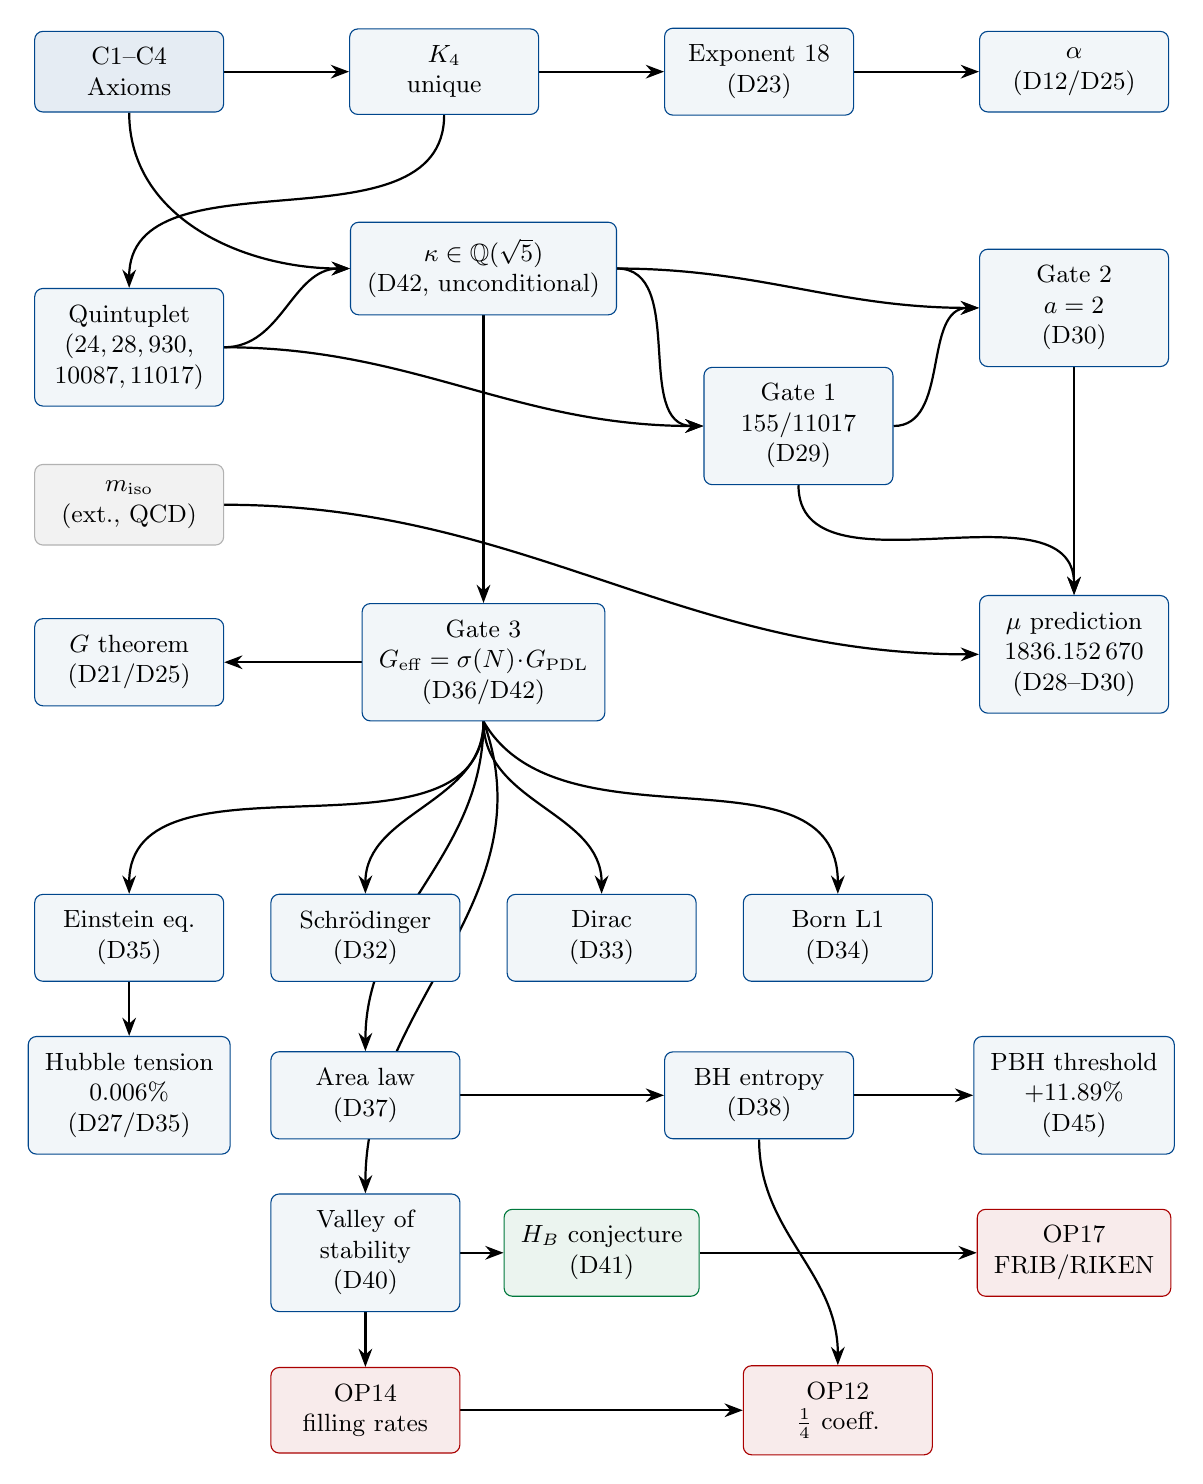
\begin{tikzpicture}[
  every node/.style={font=\small},
  axiom/.style={draw=proofblue, fill=proofblue!10,
    rounded corners=3pt, align=center, inner sep=6pt,
    minimum width=2.4cm, minimum height=0.9cm},
  theorem/.style={draw=proofblue, fill=proofblue!5,
    rounded corners=3pt, align=center, inner sep=6pt,
    minimum width=2.4cm, minimum height=0.9cm},
  conjecture/.style={draw=conjecturegreen, fill=conjecturegreen!8,
    rounded corners=3pt, align=center, inner sep=6pt,
    minimum width=2.4cm, minimum height=0.9cm},
  open/.style={draw=openproblemred, fill=openproblemred!8,
    rounded corners=3pt, align=center, inner sep=6pt,
    minimum width=2.4cm, minimum height=0.9cm},
  ext/.style={draw=gray!60, fill=gray!10,
    rounded corners=3pt, align=center, inner sep=6pt,
    minimum width=2.4cm, minimum height=0.9cm},
  arr/.style={-Stealth, thick},
]

% ── ROW 0 ── Axioms → K4 → Exp18 → alpha  (colonne gauche, y=0)
\node[axiom]   at ( 0.0,  0.0) (C1C4)      {C1--C4\\Axioms};
\node[theorem] at ( 4.0,  0.0) (K4)        {$K_4$\\unique};
\node[theorem] at ( 8.0,  0.0) (exp18)     {Exponent~18\\(D23)};
\node[theorem] at ( 12.0,  0.0) (alpha)     {$\alpha$\\(D12/D25)};

% ── ROW 1 ── Quintuplet + kappa  (y=-2.2)
\node[theorem] at ( 0.0, -3.5) (quintuplet){Quintuplet\\$(24,28,930,$\\$10087,11017)$};
\node[theorem] at ( 4.5, -2.5) (kappa)     {$\kappa\in\mathbb{Q}(\sqrt{5})$\\(D42, unconditional)};

% ── ROW 2 ── Gate1 + Gate2 + mu  (y=-2.2, colonne droite)
\node[theorem] at ( 8.5, -4.5) (Gate1)     {Gate~1\\$155/11017$\\(D29)};
\node[theorem] at (12.0, -3.0) (Gate2)     {Gate~2\\$a=2$\\(D30)};

% ── ROW 3 ── miso + G + Gate3 + mu  (y=-4.4)
\node[ext]     at ( 0.0, -5.5) (miso)      {$m_{\mathrm{iso}}$\\(ext., QCD)};
\node[theorem] at ( 0.0, -7.5) (G)         {$G$ theorem\\(D21/D25)};
\node[theorem] at ( 4.5, -7.5) (Gate3)     {Gate~3\\$G_{\mathrm{eff}}=\sigma(N)\!\cdot\!G_{\mathrm{PDL}}$\\(D36/D42)};
\node[theorem] at (12.0, -7.4) (mu)        {$\mu$ prediction\\$1836.152\,670$\\(D28--D30)};

% ── ROW 4 ── Einstein + Schrod + Dirac + Born  (y=-6.6)
\node[theorem] at ( 0.0, -11.0) (Einstein)  {Einstein eq.\\(D35)};
\node[theorem] at ( 3.0, -11.0) (Schrod)    {Schr\"odinger\\(D32)};
\node[theorem] at ( 6.0, -11.0) (Dirac)     {Dirac\\(D33)};
\node[theorem] at ( 9.0, -11.0) (Born)     {Born L1\\(D34)};

% ── ROW 5 ── Hubble + AreaLaw + BH  (y=-8.8)
\node[theorem] at ( 0.0, -13.0) (Hubble)    {Hubble tension\\$0.006\%$\\(D27/D35)};
\node[theorem] at ( 3.0, -13.0) (AreaLaw)   {Area law\\(D37)};
\node[theorem] at ( 8.0, -13.0) (BH)        {BH entropy\\(D38)};
%\node[open]    at ( 12.0, -13.0) (OP8)       {OP8\\$\varepsilon^B_G$};

% ── ROW 6 ── Nuclear + HB + OP17 + D45  (y=-11.0)
\node[theorem]    at ( 3.0,-15.0) (Nuclear){Valley of\\stability\\(D40)};
\node[conjecture] at ( 6.0,-15.0) (HB)     {$H_B$ conjecture\\(D41)};
\node[open]       at ( 12.0,-15.0) (OP17)   {OP17\\FRIB/RIKEN};
\node[theorem]    at ( 12.0,-13.0) (D45)    {PBH threshold\\$+11.89\%$\\(D45)};

% ── ROW 7 ── OP14 + OP12  (y=-13.0)
\node[open] at ( 3.0,-17.0) (OP14)         {OP14\\filling rates};
\node[open] at ( 9.0,-17.0) (OP12)         {OP12\\$\tfrac{1}{4}$ coeff.};

%% ══════════════════ FLÈCHES ══════════════════

\begin{pgfonlayer}{background}

% Row 0 — horizontales
\draw[arr] (C1C4.east)       -- (K4.west);
\draw[arr] (K4.east)         -- (exp18.west);
\draw[arr] (exp18.east)      -- (alpha.west);

% K4 → Quintuplet
\draw[arr] (K4.south)        to[out=-90, in=90] (quintuplet.north);

% Quintuplet + C1C4 → kappa
\draw[arr] (quintuplet.east) to[out=-0, in=180] (kappa.west);
\draw[arr] (C1C4.south)      to[out=-90, in=180] (kappa.west);

% kappa + Quintuplet → Gate1
\draw[arr] (kappa.east)      to[out=0, in=180] (Gate1.west);
\draw[arr] (quintuplet.east) to[out=0, in=180] (Gate1.west);

% Gate1 → Gate2, kappa → Gate2
\draw[arr] (Gate1.east)      to[out=0, in=180] (Gate2.west);
\draw[arr] (kappa.east)      to[out=0, in=180] (Gate2.west);

% kappa → Gate3
\draw[arr] (kappa.south)     -- (Gate3.north);

% Gate3 → G
\draw[arr] (Gate3.west)      to[out=180, in=0] (G.east);

% Gate1 + Gate2 + miso → mu
\draw[arr] (Gate1.south)     to[out=-90, in=90]  (mu.north);
\draw[arr] (Gate2.south)     to[out=-90, in=90]  (mu.north);
\draw[arr] (miso.east)       to[out=0,   in=180] (mu.west);

% mu → OP8
%\draw[arr] (mu.south)        to[out=-90, in=90] (OP8.north);

% Gate3 → dynamics (row 4)
\draw[arr] (Gate3.south)     to[out=-90, in=90] (Einstein.north);
\draw[arr] (Gate3.south)     to[out=-90, in=90] (Schrod.north);
\draw[arr] (Gate3.south)     to[out=-90, in=90] (Dirac.north);
\draw[arr] (Gate3.south)     to[out=-60, in=90] (Born.north);

% Einstein → Hubble
\draw[arr] (Einstein.south)  -- (Hubble.north);

% Gate3 → AreaLaw
\draw[arr] (Gate3.south)     to[out=-90, in=90] (AreaLaw.north);

% AreaLaw → BH
\draw[arr] (AreaLaw.east)    -- (BH.west);

% Gate3 → Nuclear
\draw[arr] (Gate3.south)     to[out=-70, in=90] (Nuclear.north);

% BH → OP12
\draw[arr] (BH.south)        to[out=-90, in=90] (OP12.north);

% BH → D45
\draw[arr] (BH.east)         to[out=0, in=180] (D45.west);

% Nuclear → HB → OP17
\draw[arr] (Nuclear.east)    -- (HB.west);
\draw[arr] (HB.east)         -- (OP17.west);

% Nuclear → OP14 → OP12
\draw[arr] (Nuclear.south)   -- (OP14.north);
\draw[arr] (OP14.east)       -- (OP12.west);

\end{pgfonlayer}

\end{tikzpicture}%
}
\caption{Critical-path dependency map of the PDL programme (v17).
  \textcolor{proofblue}{Blue nodes}: unconditional theorems.
  \textcolor{conjecturegreen}{Green}: conjectures.
  \textcolor{openproblemred}{Red}: open problems.
  Grey: unique external input ($m_{\mathrm{iso}}$).
  All previously conditional results are now solid arrows.
  D45 (PBH threshold) is the first falsifiable astrophysical confrontation.}
\label{fig:dependency}
\end{figure}

\newpage

% ============================================================
\section{Falsifiable Predictions}
\label{sec:predictions}

\begin{longtable}{L{0.5cm}L{3.2cm}L{5.2cm}L{4.2cm}}
\caption{Complete list of falsifiable, parameter-free PDL predictions (v17). All predictions follow from the quintuplet and $m_{\mathrm{iso}}$ alone, with no additional free parameters. Predictions P1--P6 are derived from the analytical chain; P7--P8 follow from Conjecture~$H_B$ (D41); P9 is derived from D45.}
\label{tab:predictions}\\
\toprule
\textbf{ID} & \textbf{Observable} & \textbf{PDL prediction} & \textbf{Test / status}\\
\midrule
\endfirsthead
\toprule
\textbf{ID} & \textbf{Observable} & \textbf{PDL prediction} & \textbf{Test / status}\\
\midrule
\endhead
\bottomrule
\endfoot
P1 & Proton--electron mass ratio $\mu$ & $\mu=1836.152\,670$ (parameter-free) & Testable at $0.001$~ppm; current CODATA: $1836.152\,673\,43(11)$; residual $1.8\times10^{-9}$.\\[0.4em]
P2 & Fine-structure constant $\alpha$ & $\alpha^{-1}=137.035\,999$ from quintuplet alone & Testable at $10^{-9}$; current agreement $\mathcal{O}(10^{-4})$; OP3/OP7 for residual.\\[0.4em]
P3 & Hubble constant ratio & $H_{0,\mathrm{local}}/H_{0,\mathrm{CMB}}=\sigma(N_{\mathrm{local}})/\sigma(40)$ & PDL prediction $1.085935$ vs.\ observed $1.0859\pm0.007$; $0.006\%$ error; zero free parameters.\\[0.4em]
P4 & CMB-epoch BH entropy suppression & Factor $\sigma(40)\approx 0.848$ relative to local universe & No direct observation yet; accessible via future CMB-$S_4$ constraints.\\[0.4em]
P5 & PBH survival threshold & $M^*_{\mathrm{PDL}}=\sigma(40)^{-2/3}\,M^*_{\mathrm{GR}}\approx 5.706\times10^{14}$\,g ($+11.89\%$) & Testable via Fermi-LAT IGRB analysis with \textsc{BlackHawk}/\textsc{Isatis}~\cite{D45}; excess Hawking flux at $\sim93$--$104$\,MeV.\\[0.4em]
P6 & AGN entropy-to-energy ratio & $S/E\propto G(N(z))$: systematic redshift trend & Traceable in cosmic-noon AGN surveys (JWST, Euclid); no contradicting data.\\[0.4em]
P7 & $B(E2)$ ratio in $^{90}$Ru/$^{88}$Ru & $R\approx 2.02$ (from $H_B$, $k=8\to10$) & Testable at FRIB or RIKEN; $^{88}$Ru beam available.\\[0.4em]
P8 & $N_{\mathrm{comp}}$ ratio $^{94}$Pd/$^{92}$Pd & $N_{\mathrm{comp}}(^{94}\mathrm{Pd})/N_{\mathrm{comp}}(^{92}\mathrm{Pd})=2.000\pm0.05$ & Testable from DNO-SM calculations with $^{94}$Pd spectroscopy at RIKEN.\\[0.4em]
P9 & IGRB spectral cutoff position & $E_c^{\mathrm{PDL}} \approx 93$\,MeV vs.\ $E_c^{\mathrm{GR}} \approx 104$\,MeV (shift $-10.6\%$) & Testable with Fermi-LAT IGRB data + \textsc{BlackHawk}/\textsc{Isatis}; requires non-zero $f_{\mathrm{PBH}}$ in $[5.10,\,5.71]\times10^{14}$\,g.\\[0.4em]
\end{longtable}

% ============================================================
\section{Continuation Guide}
\label{sec:continuation}

\subsection{Entry points}
\label{subsec:entrypoints}
The following entry points are recommended for a colleague wishing to contribute to specific open problems.

\begin{itemize}
\item \textbf{OP2 (global uniqueness):} Requires familiarity with D16, D16b, and combinatorial optimisation over integer lattices. The Colab infrastructure of D43 can be used to extend the computational search radius.
\item \textbf{OP4 (Born Level~2):} Requires D34 and familiarity with the Gleason theorem. The key question is the origin of $\mathrm{U}(1)$ phase freedom in the relational structure of $K_4$.
\item \textbf{OP7 (47~ppm residual in $\mu$):} Immediately actionable using the D43 Colab infrastructure. Start with the Group~I filters in D43, identify the residual at each stage, and test candidate combinatorial factors from C1--C4. Note: OP8 is resolved (D44).
\item \textbf{OP12 and OP14 (BH coefficient and filling rates):} D40 establishes that these two problems are equivalent. The recommended starting point is the coherent-configuration counting on the collective PDL surface introduced in D40, Section~4.
\item \textbf{OP16 (ZBM3--PDL):} Requires D41 and familiarity with the DNO-SM shell-model code. The formal correspondence should be established at the level of the many-body basis states, not just the eigenvalues.
\item \textbf{OP17 (FRIB/RIKEN predictions):} Experimental. Contact the PDL team before submission to ensure the prediction is correctly stated and that the appropriate source data will be requested from the experiment.
\end{itemize}

\subsection{Recommended next documents}
\label{subsec:nextdocs}
Given the current state of the programme, the following documents would have the highest impact:

\begin{enumerate}
\item \textbf{D46}: Born's rule Level~2 --- derivation of the $\mathrm{U}(1)$ phase from C1--C4 (OP4). This would complete the quantum dynamics layer.
\item \textbf{D47}: Explicit form of $C_{\mathrm{coh}}$ (OP5), enabling the first PDL computation of a gravitational wave observable.
\item \textbf{D48}: Sub-shell filling rates from axioms (OP14), which simultaneously resolves OP12 (BH coefficient $\tfrac{1}{4}$).
\item \textbf{Experimental confrontation}: Submit D45 predictions to the \textsc{BlackHawk}/\textsc{Isatis} community and contact the Fermi-LAT collaboration for a dedicated IGRB analysis in the 50--200\,MeV window. Contact F.\ Recchia and S.\ M.\ Lenzi (University of Padova) regarding P7/P8 at FRIB/RIKEN.
\item \textbf{Journal submission}: D42 (H3 theorem) or D25 (parameter-free $\alpha$--$G$ bridge) are the strongest candidates for a first peer-reviewed submission.
\end{enumerate}

% ============================================================
\section{Glossary}
\label{sec:glossary}

\begin{description}[leftmargin=3.5cm, style=nextline]
\item[AB criterion] The two-part stability criterion (amplitude condition A + balance condition B) that selects admissible two-closure couplings; proved exhaustively in D29 over $768$ configurations.
\item[Active surface $\Rsurf$] The set of valence coherence relations of the proton, $|\Rsurf|=\sigma=930$; the locus of all physical information exchange.
\item[Admissible closure] A finite signed graph satisfying all four axioms C1--C4; the minimal example is $K_4$.
\item[Born Level~1 / Level~2] Level~1: modulus rule $P=|\psi|^2$ proved via Gleason uniqueness (D34, Theorem). Level~2: derivation of the $\mathrm{U}(1)$ phase from axioms (open, OP4).
\item[$C_{\mathrm{coh}}$] Coherence stress-energy tensor appearing in the PDL Einstein equation; its explicit tensorial form is OP5.
\item[Coherence cost] Fraction of violated triangles (negative-product edges) in a signed graph; minimised by axiom C4.
\item[$\epsGeomB$] Geometric correction factor in the PDL mass-ratio formula; closed-form expression $\epsGeomB = \kappa \cdot C/(6+\kappa)\cdot(1+2/\Rtot) \in \mathbb{Q}(\sqrt{5})$ proved in D44 (OP8 resolved). The 17~ppm residual relative to CODATA reflects measurement precision of $G$.
\item[$\Geff(N)$] Effective gravitational coupling at scale $N$; equal to $\sigmaN\cdot\GPDL$ by Gate~3 (unconditional theorem).
\item[Gate 1, 2, 3] Three critical proof milestones. Gate~1: $155/11017$ from axioms (D29). Gate~2: $a=2$ from axioms (D30). Gate~3: $\Geff=\sigmaN\cdot\GPDL$ (D36/D42, now unconditional).
\item[H1, H2, H3] Named hypotheses of the programme. H1 ($\kappa=\sigma/R_{\mathrm{tot}}$): now an unconditional theorem (follows from H3/D42 via D39). H2 (bridge linearity): absorbed into D36. H3 (Indifference Lemma): proved unconditionally in D42.
\item[Indifference Lemma (H3)] The probability measure on the relations of a PDL closure is uniform; the unique measure compatible with $S_4$-symmetry of $K_4$. Proved from C1--C4 in D42 via three lemmas.
\item[$K_4$] The complete signed graph on four vertices and six edges; the unique minimal admissible closure (D16a theorem); identified with the electron prototype.
\item[$\kappa$] Primary leakage parameter; $\kappa=310\varphi/11017\in\mathbb{Q}(\sqrt{5})$; unconditional theorem of C1--C4 (D42 corollary); $\kappa\approx 0.0075194$.
\item[$m_{\mathrm{iso}}$] Isospin mass splitting $m_d-m_u$; the unique irreducible external parameter of the programme (Gate~2, D30).
\item[$N_{\mathrm{CMB}}$] PDL-derived CMB epoch parameter; $N_{\mathrm{CMB}}=40$ from neutron quintuplet (D27 theorem).
\item[OP$n$] Open Problem $n$; see Section~\ref{sec:openproblems}. OP1 fully resolved (D42).
\item[PDL] Projective Dynamic Logo; the research programme initiated in D01.
\item[Quintuplet] The integer tuple $\quintuplet$ characterising the proton; $\nu_u=24$, $\nu_d=28$, $\sigma=930$, $R_{\mathrm{sea}}=10087$, $R_{\mathrm{tot}}=11017$.
\item[$\sigmaN(N)$] Coherence engagement fraction at scale $N$; $\sigmaN=1-(1-\kappa)^N\in\mathbb{Q}(\sqrt{5})$; $\sigmaN(40)\approx 0.8449$.
\item[$\Tpp$] Proton--proton conflict unit; $C(Z>20)=190\,\Tpp$ exactly (D40 theorem).
\item[Valley of stability] Minimum neutron number $N_{\min}(Z)$ for stable nuclei; reproduced at $100\%$ accuracy for $Z=1$--82 as an unconditional theorem (D40).
\item[18-filter hierarchy] The decomposition $18=6+5+4+3$ of the leakage exponent into four topological levels (D06, D17, D23); implemented as four functional groups in D43.
\end{description}

% ============================================================
\bibliographystyle{unsrturl}
\bibliography{DM_v17_references}

\end{document}